
\chapter{Trigger Development and Performance}

\section{Introduction to Triggering}

Modern "triggering" methods began with Walther Bothe's development of the coincidence circuit. The coincidence ciruit accepts two inputs. If these inputs are recieced within the same time window, approximating coincidence, the circuit passes an output. Bothe's originally used the coincidence circuit to take data for electron-photon production in Compton scattering.

\section{Triggering at CMS}
CMS uses a two-tiered triggering system. The first tier, the L1 trigger, is hardware based. The second tier, the high-level trigger (HLT), is software based. The L1 trigger recieves raw data from the calorimeters and the muon detectors; this determines when the tracker will readout data. The raw data from the tracker, calorimeters, and muon detectors is then passed on to a computer farm running the HLT menu. The HLT then performs a simplistic reconstruction of the raw data into physics objects useful for analysis: jets, tracks, and identifiable particles. If an event passes the HLT, the raw data is permanently stored in preparation for a more complex reconstruction. 

The 2015 UPC triggers were for low multiplicity events and low transverse momentum events. Typical heavy-ion collisions are high multiplicity events. Fig.\ref{fig:eventdisplayHI} is an event display of one of the first heavy-ion collisions at CMS in 2010.

\begin{figure}[h!]
\begin{centering}
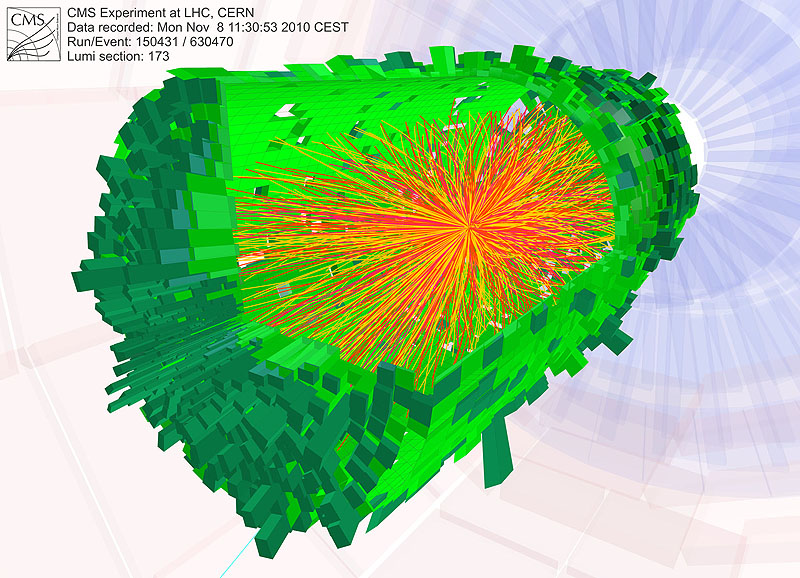
\includegraphics[width=4in]{Chapter3/importfigs/cms_firstleadcoll.jpg}
\par\end{centering}
\caption{High multiplicity PbPb collision \label{fig:eventdisplayHI}}
\end{figure}

Fig.\ref{fig:eventdisplayUPCUps} is the event display of a UPC upsilon candidate.

\begin{figure}[h!]
\begin{centering}
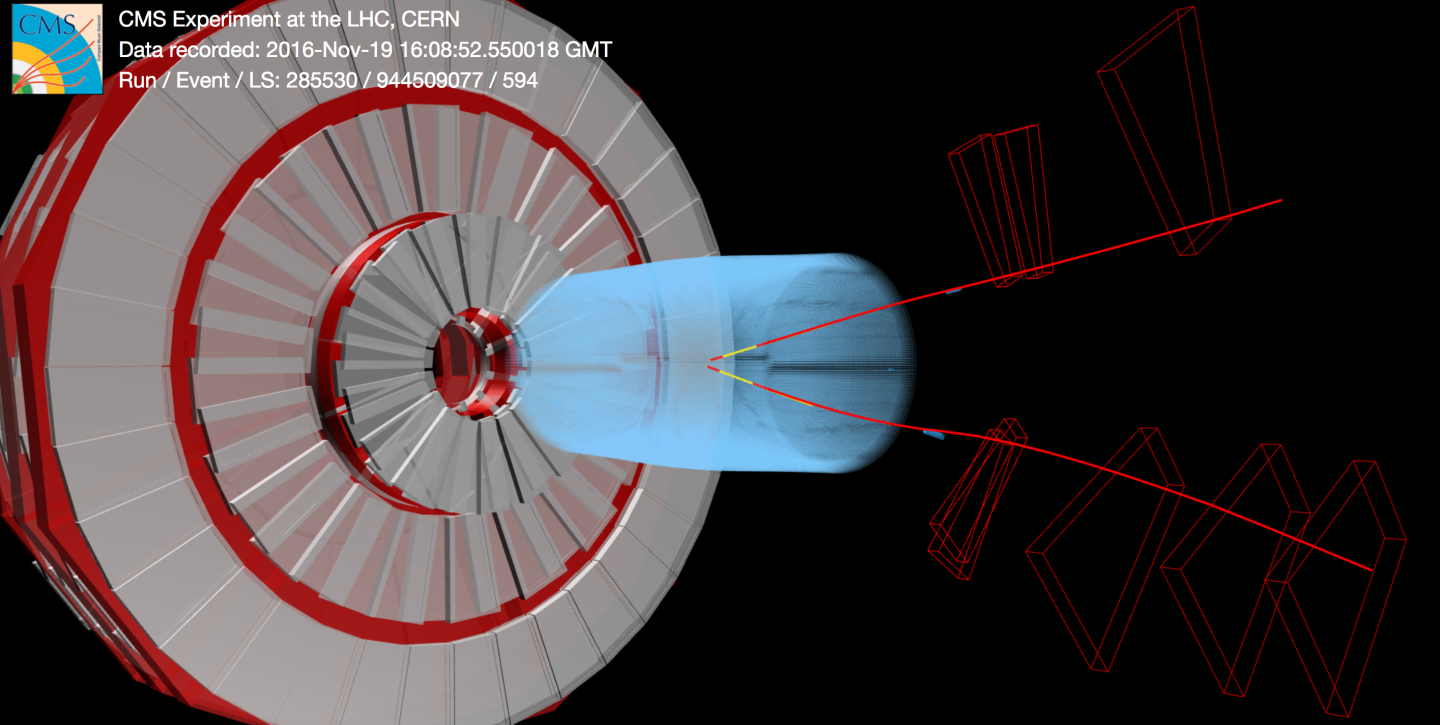
\includegraphics[width=4in]{Chapter3/importfigs/upcJpsi_run285530_lumi594_event944509077_v0.png}
\par\end{centering}
\caption{UPC Upsilon candidate \label{fig:eventdisplayUPCUps}}
\end{figure}

For this analysis, the L1 trigger applies two selections. First, the L1 checks that at least one of the HF is empty. This is the most important part of the trigger in so far as it suppressed the hadronic contamination of the dataset. Then, if there is at least 5 GeV of energy deposited in the ECAL, the event passes to the HLT. 

Low multiplicity events are difficult to distinguish from background. To compensate, the HLT in turn requires that there be at least once reconstructed track from the pixel tracker, to make sure that there are particles that will be reconstructed by the complete tracker. Only the pixel tracker is used for these HLTs to increase the speed of reconstruction while decreasing needed computer cycles. 

\begin{figure}[h!]
\begin{centering}
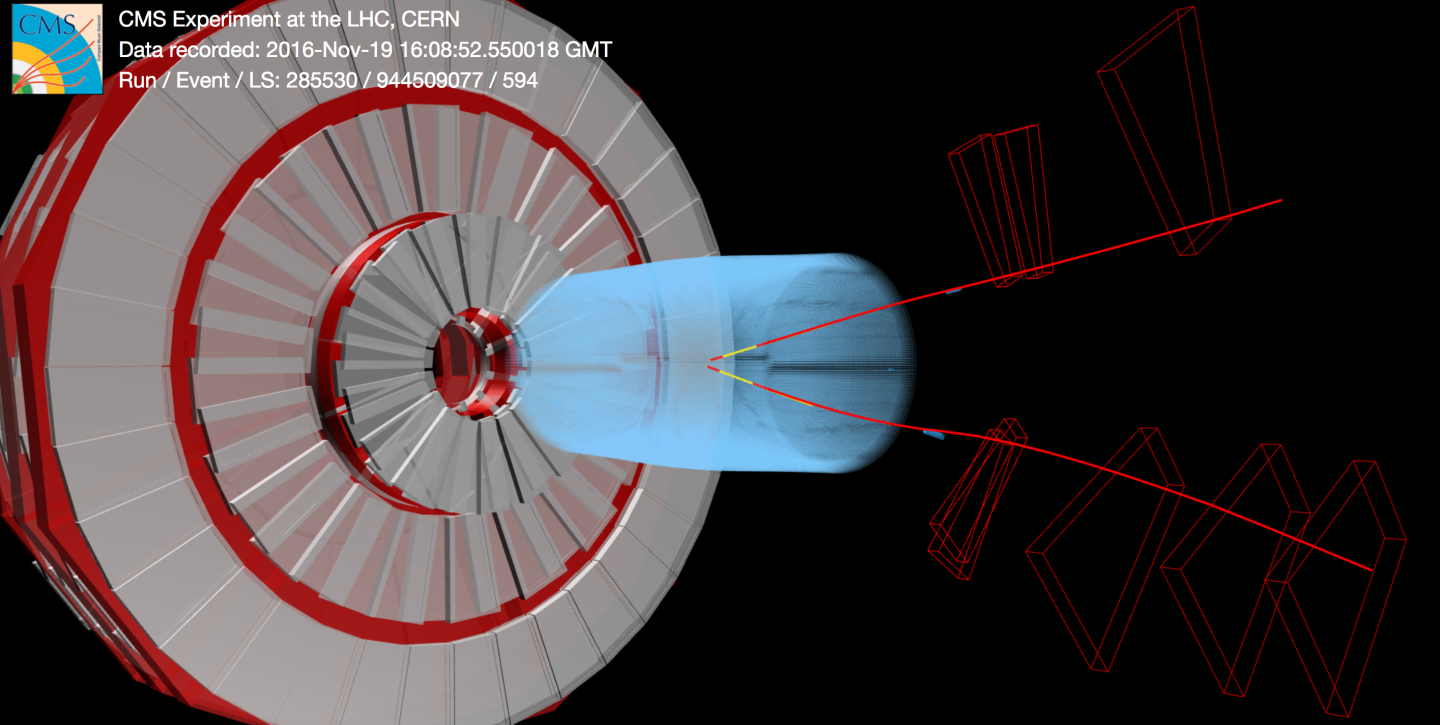
\includegraphics[width=4in]{Chapter3/importfigs/upcJpsi_run285530_lumi594_event944509077_v0.png}
\par\end{centering}
\caption{UPC Upsilon candidate \label{fig:eventdisplayUPCUps}}
\end{figure}


\section{My Contributions}

In preparation for the 2015 heavy-ion run, I prepared a high-level trigger menu. This trigger menu was optimized for firing on ultra-peripheral collisions. I tested the menu's performance on Monte Carlo generated by STARLIGHT and reconstructed through a GEANT4 simulation of CMS. During the experiment, I was present at CERN to monitor the trigger rates and deliver daily reports on their performance. 

\begin{figure}[h!]
\begin{centering}
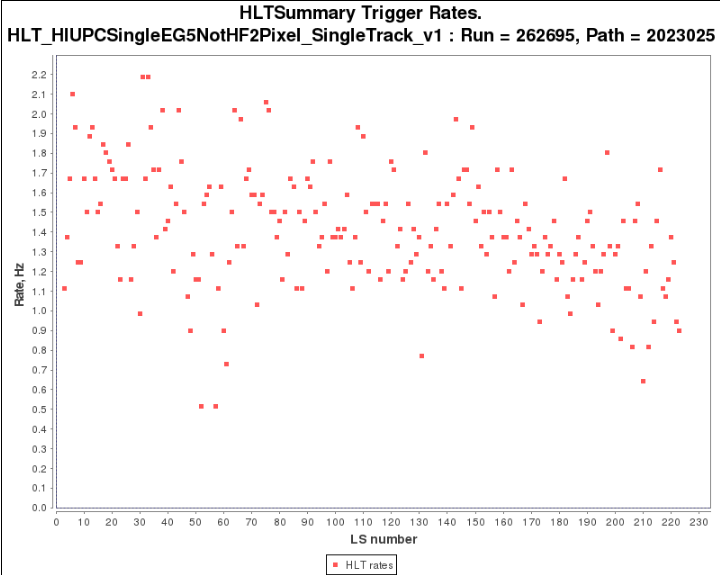
\includegraphics[width=4in]{Chapter5/importfigs/triggerRateExample.png}
\par\end{centering}
\caption{Example of trigger rate. \label{fig:trigRate}}
\end{figure}

